\documentclass[]{book} % fleqn/leqno

\usepackage{makeidx} \makeindex
\usepackage{lipsum}
\usepackage{hyperref}
\usepackage{tabularx}
\usepackage{multirow}
\usepackage{lipsum}
\usepackage[table]{xcolor}
\usepackage{graphicx}


\renewcommand*\contentsname{A new name for list of contents}
\renewcommand{\listfigurename}{A new name for list of figures}
\renewcommand{\listtablename}{A new name for list of tables}

\begin{document}

\tableofcontents \newpage
\listoffigures \newpage
\listoftables \newpage

\chapter{Chapter name}

\section{Introduction}\label{sec:intro}

\lipsum[1] 

You can see it in Section \ref{sec:sth}.

\section{Something Else}\label{sec:sth}

As you see it in Section \ref{sec:intro}, \lipsum[1]

\section{Examples}

\lipsum \index{blah blah|(}

\subsection{Example of Table}

\begin{table}[!h]
\centering
\begin{tabular}{|c|c|c|}
	\hline 
	\multicolumn{3}{|c|}{Multiple Column} \\
	\hline 
	A &  B & C \\
	\hline 
	\multirow{3}{*}{Multiple row} & Cell 1 & Cell 2 \\
	& Cell 3 & Cell 4 \\
	& Cell 5 & Cell 6 \\
	& Cell 7 & Cell 8 \\
	\hline
 \end{tabular}
\caption{Using multirow and multicolumn}
\label{tab:multi}
\end{table}

\subsection{Example of Figure}

\lipsum \index{turing}

\begin{figure}[!h]
	\centering
    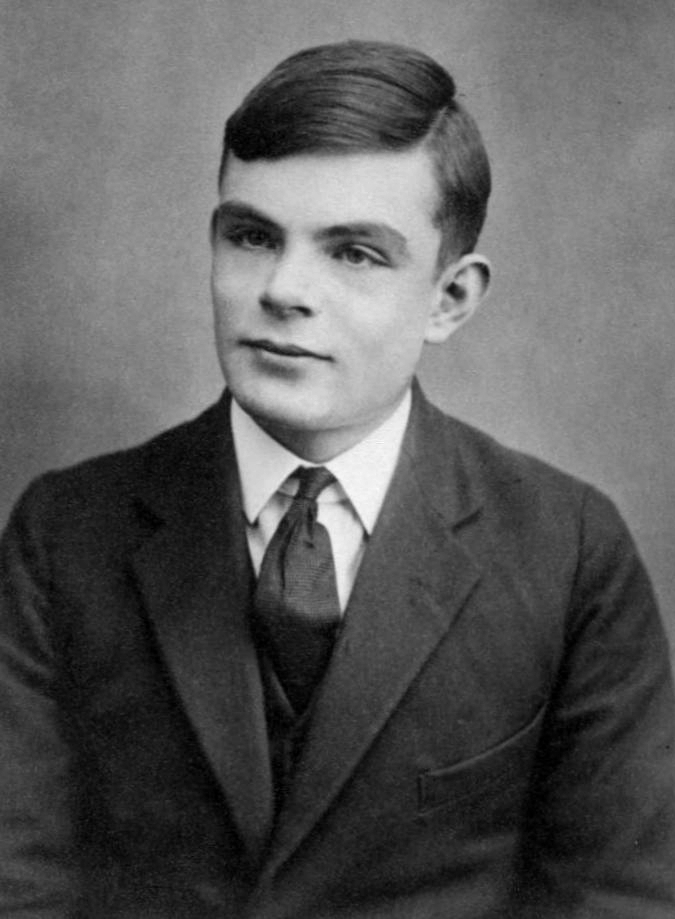
\includegraphics[width=0.5\linewidth]{Turing.jpeg}
    \caption[Turing]{Alan Turing}
	\label{fig:turing}
\end{figure}

\clearpage

\begin{figure}[!h]
	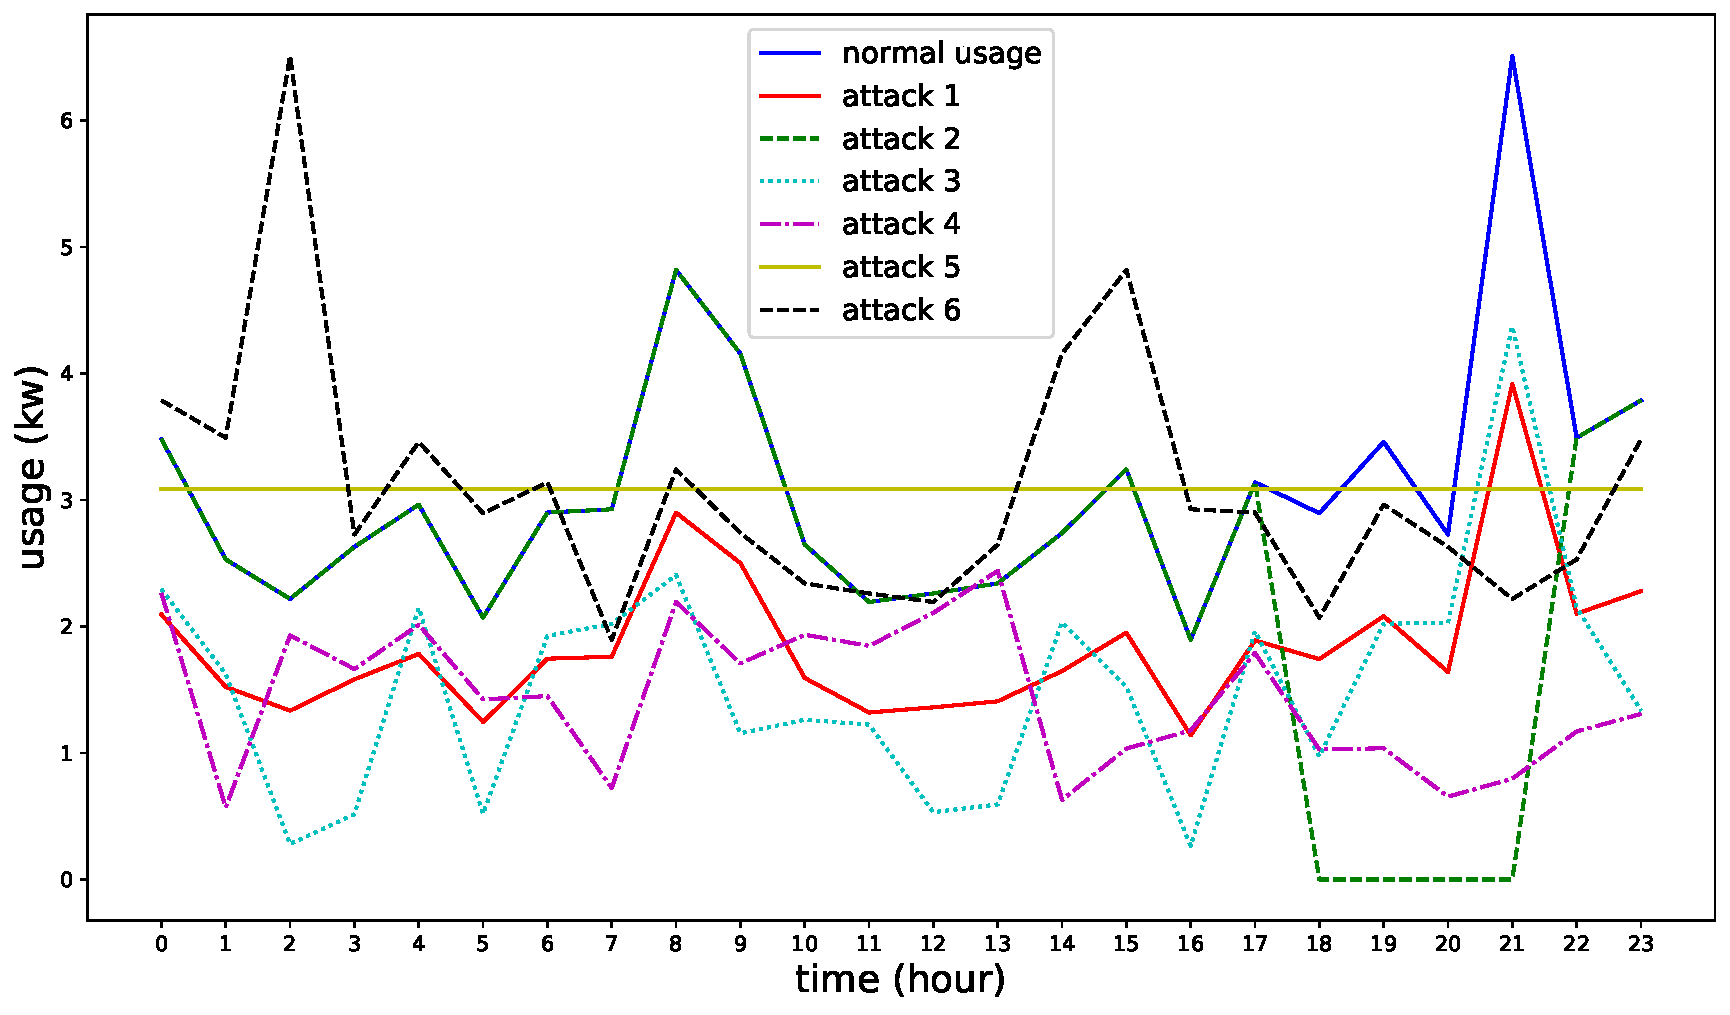
\includegraphics[width=\linewidth,scale=1]{attack.pdf}
	\caption{A figure from article \cite{tehrani2020decision}}
	\label{fig:attack}
\end{figure}

\lipsum \index{blah blah|)}

You can check Figure \ref{fig:turing}, Figure \ref{fig:attack}, and Table \ref{tab:multi}.


\clearpage
\bibliographystyle{plain}
\bibliography{mybibfile}

\printindex
\end{document}